\documentclass[12pt, a4paper]{article}

\usepackage[utf8x]{inputenc}
\usepackage[lithuanian]{babel}
\usepackage[L7x]{fontenc}
\usepackage{lmodern}
\usepackage{verbatim}
\usepackage{tocloft} 
\usepackage{url}
\usepackage{setspace}
\usepackage{caption}
\usepackage{parskip}
\usepackage{graphicx}
\usepackage{fixltx2e} % šitas dėl \textsubscript{}
\usepackage{color} % spalvinsim tekstą
\usepackage{mathtools} % pades rašyti matematinius intarpus
\usepackage{titlesec}
\usepackage{indentfirst} % atitraukta pirmoji eilute
\usepackage{longtable} % darysim didelias lenteles
\usepackage{algorithm}
\usepackage{lipsum}% http://ctan.org/pkg/lipsum
\usepackage[top=2cm, bottom=2cm, left=3cm, right=1.5cm]{geometry}
\usepackage{changepage}
\usepackage{pdfpages} % su šitua paketu galima įkelti pdf kaip puslapius
\linespread{1.5}
\parindent = 1cm
\titlelabel{\thetitle.\quad} % Padeda tašką po skyriaus numerio
\renewcommand{\cftsecleader}{\cftdotfill{\cftdotsep}}

\begin{document}
% Titulinis puslapis
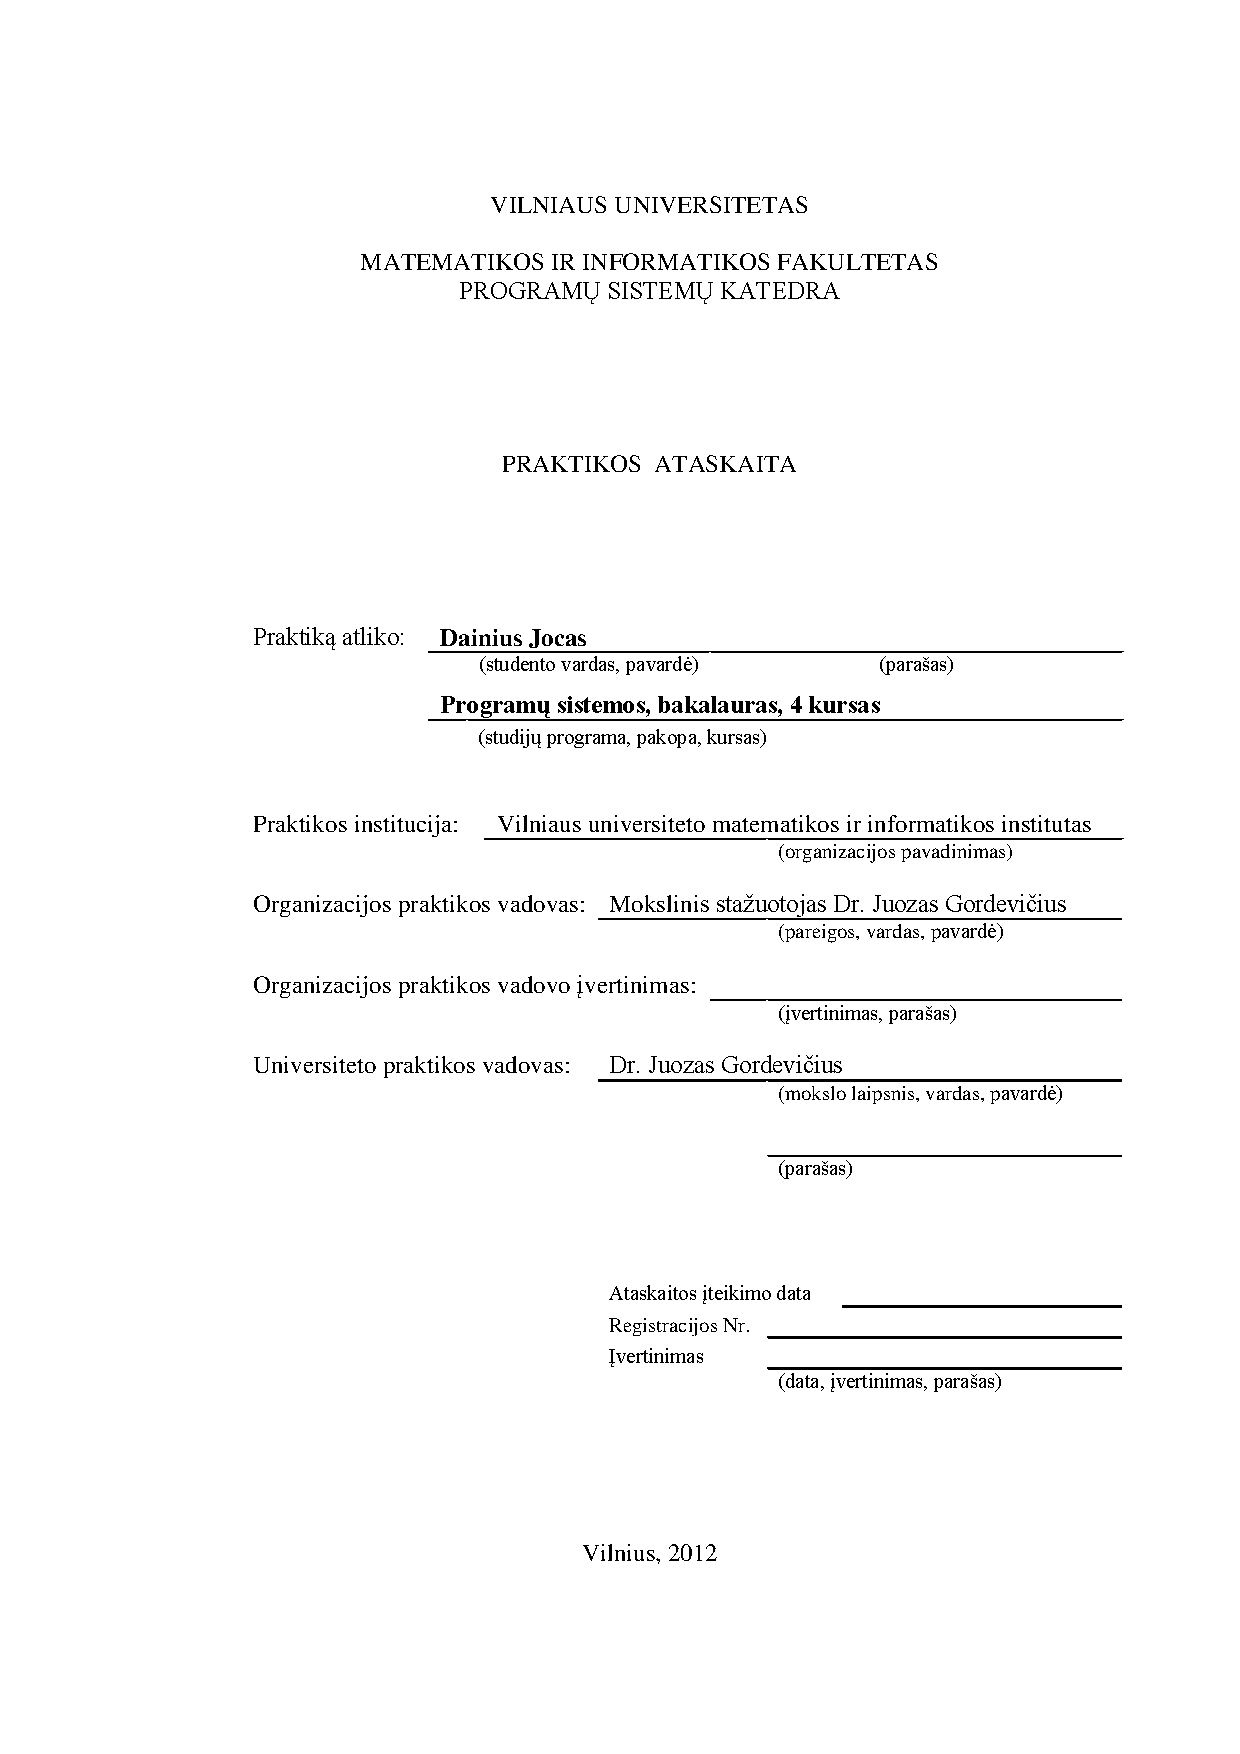
\includepdf{images/praktikos_ataskaitos_titulinis.pdf}

\let \savenumberline \numberline
\def \numberline#1{\savenumberline{#1.}}
\tableofcontents 
\newpage

%% Įvade aprašomi darbo tikslai, nurodomas temos aktualumas, aptariamos teorinės darbo prielaidos bei metodika, apibrėžiamas tiriamasis objektas, apibūdinami su tema susiję literatūros ar kitokie šaltiniai, temos analizės tvarka, darbo atlikimo aplinkybės, pateikiama žinių apie naudojamus instrumentus (programas ir kt.). Darbo įvadas neturi būti dėstymo santrauka. Įvado apimtis 3–4 puslapiai.

\newpage
\section*{ĮVADAS}

%% JG: Idėja - naudok terminus "matai" ir "mėginiai". Kiekvienam mėginiui atliekama labai daug matavimų, iš to ir "daugiamatiškumas"

% JG: Paminėk, kad šiame darbe mes gilinamės į biomedicinoje kaupiamų genetinių duomenų analizės specifika. Šie duomenys ypatingi dėl daugiamatiškumo, mažo mėginių kiekio, triukšmingų matavimų.

Nuolat vystosi technologijos skirtos gauti biomedicininius duomenis, pvz. genomo sekvenavimas\cite{pettersson2009generations}, o tai reiškia, kad didėja gaunamų duomenų detalumas. Detalumas reiškia, kad daugėja biomedicininius duomenis abibūdinančių faktorių arba matų skaičius. Duomenys, kurių kiekvienas mėginys aprašomas dideliu skaičiumi matų, yra vadinami daugiamačiais duomenimis.

Šiame darbe yra nagrinėjama biomedicinoje kaupiamų genetinių daugiamačių duomenų analizės specifika. Šie duomenys yra specifiški tuo, kad jie įprastai turi šimtus kartų daugiau matų nei mėginių. Kadangi mėginio gavimo kaina yra aukšta, turimas mažas mėginių skaičius. Biomedicininių duomenų analizę apsunkina ir tai, kad matavimai, kuriais tie duomenys gaunami, yra triukšmingi. Triukšmas matavimo metu atsiranda dėl cheminių reakcijų netikslumo, tiriamo organizmo sudėtingumo. Kai duomenys yra triukšmingi ir didėja juos apibūdinančių matų skaičius, didėja tikimybė duomenyse bus rasta atsitiktinių priklausomybių. Tai yra pagrindinė priežastis, kodėl biomedicininių duomenų analizės procesas yra sudėtingas.

%% JG: Būdai neatsiranda, o vystosi technologija. Jie nėra tikslesni, bet detalesni, t.y. kiekvienam mėginiui atliekama daugiau matavimų. 

%% JG: Nors matavimų kiekis didėja, mėginio kaina išlieka gana aukšta. Todėl biomedicinos eksperimentuose gaunami duomenys ypatingi tuo, kad matų visados ženkliai daugiau nei mėginių.

Biomedicininių duomenų klasifikavimo užduotis yra atskirti sveikųjų pacientų mėginius nuo sergančiųjų. Klasifikavimu siekiama nustatyti, kurie matai, veikdami drauge, geriausiai paaiškina skirtumą tarp ligos paveiktų ir nepaveiktų mėginių. Labiausiai ligą paaiškinančių matų nustatymas galėtų palengvinti tiriamų ligų diagnozės ir gydymo metodų kūrimą. Klasifikavimu yra vadinamas duomenų analizės procesas, kurio metu yra sukonstruojama funkcija, atskirianti duomenis į grupes (arba klases) pagal jų matus \cite{fisher1936use}. Sukonstruotos funkcijos yra vadinamos klasifikatoriais, o jų konstravimo algoritmai -- klasifikavimo algoritmais. Klasifikatoriai paruošiami naudojant turimus mėginius -- treniravimosi duomenis -- ir informaciją apie jų būklę (sveikas ar sergantis). Klasifikatoriaus ruošimo procesas yra vadinamas apmokymu. Klasifikatoriai yra validuojami su testiniais duomenimis Klasifikatoriai naudojami nustatant naujų, dar nematytų, mėginių būklę.

Dėl ,,daugiamatiškumo prakeiksmo`` (angl. \textit{the curse of dimentionality}) didėjant matų kiekiui mėginiai pasidaro panašūs, todėl bandymas juos klasifikuoti tolygus spėliojimui \cite{bellman1966adaptive}. Biomedicininių duomenų kontekste galima daryti prielaidą, kad ne visi matai yra susiję su tiriama problema, pvz. gaubtinės žarnos vėžiu, dėl to, kad duomenys yra daugiamačiai. Paprastai nagrinėjamai problemai svarbus yra mažas, palyginus su visu, matų kiekis.  Todėl biomedicininių duomenų daugiamatiškumui sumažinti yra naudojami informatyviausių matų atrinkimo metodai \cite{guyon2003introduction} (angl. \textit{feature selection}). Pagal tai, kaip susiję su klasifikatoriumi, matų atrinkimo metodai skirstomi į tris kategorijas \cite{saeys2008robust}: filtruojantys (angl. \textit{filter}), prisitaikantys (angl. \textit{wrapper}) ir įterptiniai (angl. \textit{embedded}) metodai. Filtruojančiais metodais pirmiausia yra atrenkami informatyviausi matai, o tada apmokomas klasifikatorius. Prisitaikančiųjų 
metodų atveju, pirma, apmokomas klasifikatorius su visais matais, antra, parenkamas matų poaibis ir apmokomas klasifikatorius, tada po daugkartinio matų aibių įvertinimo pagal klasifikavimo rezultatus yra nusprendžiama, kuris matų poaibis yra labiausiai tinkamas klasifikavimui. Įterptinių metodų atveju matų atrinkimo procesas yra neatsiejamas nuo klasifikavimo proceso -- pats klasifikatorius įvertina matus.

Matų atrinkimas yra svarbi biomedicininių duomenų apdorojimo (angl. \textit{preprocessing}) etapo dalis. Naudojant matų atrinkimo metodus, galima kovoti su daugiamatiškumo prakeiksmu matų skaičių priartinant prie mėginių skaičiaus. Todėl svarbu yra pasirinkti geriausiai tinkančią matų atrinkimo strategiją. Kadangi ir pačių matų atrinkimo metodų veikimas priklauso nuo konkrečių duomenų, tai paties matų atrinkimo metodo pasirinkimas yra sudėtinga užduotis. 

Dirbant su biomediciniais duomenimis dažniausiai turime tik kelias dešimtis mėginių, todėl, norint geriau įvertinti klasifikatoriaus tikslumą, yra naudojami pakartotinio mėginių poaibio atrinkimo (angl. \textit{resampling}) metodai: kryžminio patikrinimo (angl. \textit{cross-validation}) arba įkelčių (angl. \textit{bootstrap\footnote{Terminas \textit{bootstrap} ,,įkelties`` prasme pradėtas naudoti dar Rudolfo Ericho Raspės knygoje ,,Barono Miunchauzeno nuotykiai``(1785), kurioje Baronas Minchauzenas užkėlė save ant arklio tempdamas į viršų savo batų raištelius (angl. \textit{bootstraps}).}}). Šių metodų naudojimas su duomenimis, kurių tikrasis pasiskirstymas nėra žinomas, padeda įvertinti klasifikavimo rezultatų variabilumą (angl. \textit{variance}) ir sisteminį nuokrypį (angl. \textit{bias}).

Naudojant kryžminio patikrinimo metodą, daug kartų sudaromos skirtingos treniravimosi ir testinės mėginių imtys. Taikant atskirą šio metodo variantą, kryžminį patikrinimą išbraukiant po vieną mėginį (angl. \textit{leave-one-out cross-validation}), iš treniravimosi imties išbraukiamas vienas mėginys ir apmokomas klasifikatorius, kuris klasifikuoja išbrauktąjį mėginį. Procesas tęsiamas tol, kol suklasifikuojami visi objektai. Kitais kryžminio patikrinimo metodo variantais iš treniravimosi mėginių yra išmetama po keletą mėginių. Pagal tai, kiek testinių mėginių klasifikatorius priskyrė klaidingai kategorijai, yra nustatoma vidutinė klaidingo klasifikavimo tikimybė. Šiuo metodu gauti įverčiai pasižymi dideliu klasifikavimo rezultatų variabilumu \cite{braga2004cross}.

Naudojant įkelčių metodą, iš $n$ dydžio mėginių aibės yra paimama tokio pačio dydžio atsitiktinių mėginių imtis su pasikartojimais, kuri vadinama įkelties treniravimosi imtimi. Į šią imtį nepaimti mėginiai yra priskiriami testavimo imčiai. Naudojant įkelties treniravimosi mėginių imtį yra apmokomas klasifikatorius, kuris klasifikuoja testavimo imtį. Procesą kartojant gaunama klaidingo klasifikavimo tikimybės įverčių imtis. Šios imties vidurkis yra klaidingo klasifikavimo tikimybės įvertis. Dažniausiai naudojamas ,“0.623 įkelčių`` (angl. \textit{0.623\footnote{0.623 yra tikimybė mėginiui būti įtrauktam į treniravimosi imtį.} bootstrap}) įverčiu. Šiuo metodu gautas klaidingo klasifikavimo tikimybės įverti pasižymi mažu klasisifikavimo rezultatų variabilumu \cite{michie1994machine}.

%% JG: Kodėl klasifikuojama? Norima nustatyti, kokie matai, veikdami drauge, geriausiai paaiškina skirtumą tarp ligos paveiktų ir sveikų mėginių.

%% JG: Kokios yra tradicinės klasifikavimo strategijos ir kodėl jos neveikia daugiamačių duomenų atveju? Skaičiavimo laikas nėra problema - Random forests veikia visai neblogai tokiais atvejais. Daugiamatiškumas veda prie the curse fo dimensionality.

% JG: sumažinus naudojamų matų kiekį, matų kiekis priartėja prie mėginių kiekio ir tokiu būdu apeinamas daugiamatiškumo prakeiksmo problema. Biomedicinos duomenų kontekste, galima daryti prielaidą, kad dauguma matų yra beprasmiai, pvz., tik kai kurie genai įtakoja ligą, todėl matų mažinimimas yra prasmingas. Taip pat, kuriant medicininius diagnostikos įrankius, naudojamų matų kiekis įtakoja įrankio kainą. Todėl pageidautina turėti kuo mažiau matų.

Kadangi biomedicininiuose duomenyse reikšmingų matų kiekis tiriamai problemai yra nedidelis, todėl tyrėjams norint geriau suprasti nagrinėjamus biomedicininius duomenis yra svarbu orientuotis į mažesnį matų poaibį, kuris yra svarbus nagrinėjamai problemai. Tokioje situacijoje tampa svarbu, kaip varijuoja atrenkamų matų aibė, kai matų atrinkimas vykdomas su vis kitu mėginių poaibiu. Matai, kurie keičiant mėginių, naudojamų matų atrinkime, poaibį yra vėl ir vėl atrenkami, yra vadinami stabiliais matais \cite{devijver1982pattern}. Parametras, parodantis kaip stabiliai yra atrenkami matai, yra vadinamas stabilumu \textit{(angl. robustness)}. Tačiau skirtingi matų atrinkimo metodai tiems patiems mėginiams gali atrinkti skirtingus matus. Taip pat, suskaidžius duomenis į persidengiančius poaibius ir atrinkus tą patį kiekį matų tuo pačiu metodu, gaunamas skirtingas matų poaibis. Matų aibės sumažinimas paspartina biomedicininių duomenų tyrimus -- tyrėjams reikia atlikinėti bandymus su mažesniu mėginių skaičiumi. 
Kuriant medicininius diagnostikos įrankius, naudojamų matų kiekis įtakoja įrankio kainą. Todėl stabilių matų atrinkimas dirbant su biomedicininiais duomenimis yra svarbus.

% JG: Žiūrėkim į stabilumą kaip į šalutinį matų atrinkimo efektą, kurį svarbu pažaboti. Stabilumas svarbus, nes, analizuojant duomenis norima ne tik nustatyti, koks būtų vidutinis klasifikatoriaus tikslumas, bet ir sukurti tą vidutinį klasifikatorių. Norint pastarąjį sukurti, reikia žinoti, kuriuos konkrečius matus naudoti. 

% JG: Šitam paragrafe suplaki daug svarbių dalykų į krūvą ir juos turėtum būti paaiškinęs jau anksčiau. Mėginių trūkumas nėra tavo sprendžiama problema. Tačiau, kuo mažiau duomenų, tuo nestabilesni atrenkami matai. 

%Taigi, dirbant su daugiamačiais duomenimis, reikia atsižvelgti į keletą kriterijų:
%\begin{enumerate}
% \item Klasifikavimo tikslumą;
% \item Matų atrinkimo stabilumą, atsižvelgiant į klasifikavimo rezultatus;
% \item Triukšmo lygį duomenyse;
% \item Skaičiavimo išteklių naudojimo racionalumą.
%\end{enumerate}
%Reikalavimas vienu metu atsižvelgti į keletą kriterijų užduotį daro sudėtinga. Klasifikuojant daugiamačius duomenis uždavinys yra surasti geriausius rezultatus duodančią strategiją, kuri geriausiai atsižvelgia į minėtus kriterijus.

%Darbo eksperimentinei daliai reikalingus skaičiavimo išteklius, suteikė VU MIF skaitmeninių tyrimų ir skaičiavimų centras \cite{mif2012stsc}. Eksperimentuose buvo naudojami laisvai internete prieinami biomedicininių duomenų rinkiniai (angl. \textit{datasets}). Biomedicininių duomenų apdorojimo algoritmų implementavimui buvo naudojama R \cite{r2012statistics} programavimo kalba. Eksperimentai atlikti profesinės praktikos MII metu.

Matų atrinkimo stabilumo problemą Yang ir Mao \cite{yang2011robust} siūlė spręsti reitinguojant matus remiantis keletos matų atrinkimo metodų rezultatais. Galutinis matų reitingo sąrašas gaunamas, kai po kiekvieno matų atrinkimo yra išmetama viena žemiausią reitingą turintis matas iš matų aibės, ir matų atrinkimas yra kartojamas tol, kol nebelieka matų. Tačiau matų atrinkimo metodų kiekis yra ribotas ir skirtingų metodų dažnai negalima vykdyti išskirstytų skaičiavimų aplinkoje. Tai riboja šio metodo pritaikomumą daugiamačių duomenų analizėje.

Matų atrinkimo stabilumo problemą siūlyta spręsti surandant matų grupių tankio centrus ir naudoti matus, kurie artimiausi tiems centrams \cite{yu2008stable}. Pasiūlytas grupių tankių algoritmas užtrunka $O(\lambda n^2m)$ laiko, kur $n$ yra matų kiekis, o $m$ - mėginių skaičius. Vėliau Loscalzo ir kt. pasiūlė mokymo duomenis skaidyti poaibiais ir kiekviename poaibyje ieškoti tankių grupių, o tada imti sprendimą balsavimo principu \cite{loscalzo2009consensus}. Nors šie metodai siūlo stabilų matų atrinkimą, tačiau šių metodų panaudojamumą daugiamačiuose duomenyse riboja skaičiavimo sudėtingumas.

Šiame bakalauriniame darbe remiantis Yang, Mao bei Loscalzo darbuose pateiktomis įžvalgomis, bus stengiamasi pasiūlyti tyrimų kryptis, kurios galėtų padėtų sukurti metodus, skirtus spręsti stabilių matų atrinkimo problemą. Idėja yra sugrupuoti matus pagal greitą klasterizacijos algoritmą, išrinkti reprezentatyviausius matus, transformuoti matų erdvę ir joje vykdyti matų atrinkimą remiantis keletu matų atrinkimo metodų.

Šio darbo tikslas yra išanalizuoti darbo su daugiamačiais duomenis ypatybes. Šiam darbui yra keliamos tokios užduotys:
\begin{enumerate}
 \item Susipažinti su naujausiais klasifikavimo ir matų atrinkimo metodais;
 \item Atlikti matų atrinkimo metodų palyginamuosius eksperimentus;
 \item Pasiūlyti kryptis, kaip dabartiniai metodai gali būti patobulinti ir paruošti naujųjų metodų prototipus.
\end{enumerate}

Tolimesnė bakalaurinio darbo struktūra yra tokia: skyriuje


\newpage

% 2.	Įmonės/įstaigos apibūdinimas. Glaustai aprašoma įmonė/įstaiga, kurioje buvo
% atliekta praktika: jos veiklos sritis, organizacinė struktūra, teikiamos 
% paslaugos ir kt. Apibūdinamos praktikos vietoje sudarytos darbo sąlygos
% (1-2 psl.).

\section{Įstaigos apibūdinimas}

Vilniaus universiteto matematikos ir informatikos institutas (MII) nuo 2010 m. yra Vilniaus 
universiteto padalinys užsiimantis tyrimais matematikos ir informatikos srityse.
Instituto įkūrimo data laikoma 1965 m. spalio 1d., kai buvo panaikintas Lietuvos
mokslų akademijos Fizikos ir technikos institutas ir įkurti trys nauji
institutai, tarp kurių buvo Fizikos ir matematikos institutas, kuris laikomas 
MII pirmtaku. 

Pagrindinė instituto veikla - moksliniai tyrimai ir eksperimentinė plėtra. Kitos
veiklos sritys yra: mokslininkų ugdymas (doktorantūros studijos); mokslo 
organizacinė veikla; leidyba; mokymas, moksleivių ugdymas, švietimas.
Mokslinė veikla sukoncentruota 11-oje mokslinių padalinių. Institute yra 5
matematikos krypties padaliniai, 7 informatikos bei informatikos inžinerijos 
padaliniai:
\begin{enumerate}
  \item Atpažinimo procesų skyrius;
  \item Atsitiktinių procesų skyrius;
  \item Informatikos metodologijos skyrius;
  \item Kompiuterinių tinklų laboratorija;
  \item Matematinės logikos sektorius;
  \item Programų sistemų inžinerijos skyrius;
  \item Sistemų analizės skyrius (SAS);
  \item SAS optimizavimo sektorius;
  \item SAS operacijų tyrimo sektorius;
  \item Skaičiavimo metodų skyrius (SMS);
  \item SMS diferencialinių lygčių sektorius;
  \item Tikimybių teorijos ir statistikos skyrius;
\end{enumerate}

MII man, kaip ir kiekvienam darbuotojui, parūpino: darbo vietą, prisijungimo prie 
vietinio tinklo, galimybe naudotis skaičiavimo ištekliais, galimybe su nuolaida 
pietauti vietinėje valgykloje. MII darbuotojai buvo kolegiški, todėl apsipratimas
MII įvyko labai greitai. Todėl jau nuo pat pirmosios profesinės praktikos dienos
galėjau pradėti spręsti užsibrėžtus uždavinius.

\newpage

%% Praktikos veiklos aprašymas (vienas arba keli skyriai). Aprašomas praktikos užduoties įgyvendinimas (pvz., atlikti projektavimo ir/ar programavimo darbai, sukurtas modelis, priimti sprendimai ir pan.).

\section{PROFESINĖS PRAKTIKOS VEIKLOS APRAŠYMAS}
\label{praktikos_veiklos_aprasymas}

Šiame skyriuje aprašysiu profesinės praktikos veiklas, kurias skirsčiau į užduotis. Profesinę praktiką sudarė trys užduotys: susipažinimas su daugiamačių duomenų dimensijų atrinkimo problematika, dimensijų atrinkimo metodų programavimas ir dimensijų atrinkimo metodų savybių tyrimas. Toliau šiame skyriuje aprašysiu kiekvieną užduotį atskirai.

\subsection{Įvadas į profesinės praktikos metu nagrinėtą problematiką ir literatūros apžvalga}

Nuolat vystosi technologijos skirtos gauti biomedicininius duomenis, pvz. genomo sekvenavimas \cite{pettersson2009generations}, o tai reiškia, kad didėja gaunamų duomenų detalumas. Detalumas reiškia, kad daugėja biomedicininius duomenis abibūdinančių faktorių arba matų skaičius. Duomenys, kur kiekvienas mėginys aprašomas dideliu kiekiu matų, yra vadinami daugiamačiais duomenimis.

Šiame darbe yra nagrinėjama biomedicinoje kaupiamų genetinių daugiamačių duomenų analizės specifika. Šie duomenys yra ypatingi tuo, kad jie įprastai turi šimtus kartų daugiau matų nei mėginių. Santykinai mažas mėginių skaičius turimas, nes mėginio gavimo kaina yra aukšta. Biomedicininių duomenų analizę apsunkina ir tai, kad matavimai, kuriais tie duomenys gaunami, įneša atsitiktinių duomenų - triukšmo. Triukšmas matavimo metu gali atsirasti dėl įvairių priežasčių, pvz. netinkamai paruoštų cheminių preparatų. Kai duomenys yra triukšmingi, didėja tikimybė duomenyse rasti atsitiktinių priklausomybių. Tai yra viena priežasčių, kodėl biomedicininių duomenų analizės procesas yra sudėtingas.

Klasifikavimu \cite{fisher1936use} yra vadinamas duomenų analizės procesas, kai duomenys suskirstomi į grupes pagal tam tikrus jų požymius. Algoritmai arba funkcijos, kurios turimus duomenis priskiria iš anksto žinomoms grupėms - atlieka klasifikavimą - yra vadinami klasifikatoriais. Klasifikatoriai paruošiami naudojant turimus mėginius - treniravimosi duomenis - ir informaciją apie jų būklę (sveikas ar sergantis). Klasifikatoriaus ruošimo procesas yra vadinamas apmokymu. Apmokyti klasifikatoriai paprastai naudojami nustatant naujų, dar nematytų, mėginių būklę. Biomedicininių duomenų klasifikavimo tipinė užduotis yra atskirti sveikų pacientų mėginius nuo sergančiųjų. Klasifikavimu siekiama nustatyti, kurie matai veikdami drauge, geriausiai paaiškina skirtumą tarp ligos paveiktų ir sveikų mėginių. Labiausiai ligą paaiškinančių matų nustatymas galėtų palengvinti tiriamų ligų diagnozės ir gydymo metodų kūrimą.

Biomedicininių duomenų kontekste galima daryti prielaidą, kad ne visi matai yra susiję su tiriama problema, pvz. gaubtinės žarnos vėžiu, dėl tokių faktorių, kaip triukšmas duomenyse. Paprastai nagrinėjamai problemai svarbus yra mažas, palyginus su visu, matų kiekis. Ši biomedicininių duomenų ypatybė veda prie ,,daugiamatiškumo prakeiksmo`` (angl. \textit{the curse of dimentionality}) \cite{bellman1966adaptive} - didėjant matų kiekiui mėginiai pasidaro panašūs, todėl bandymas juos klasifikuoti tolygus spėliojimui. Todėl biomedicininių duomenų daugiamatiškumui sumažinti yra naudojami informatyviausių dimensijų atrinkimo metodai \cite{guyon2003introduction} (angl. \textit{feature selection}). Pagal tai, kaip susiję su klasifikatoriumi, dimensijų atrinkimo metodai skirstomi į tris kategorijas \cite{saeys2008robust}: filtruojantys (angl. \textit{filter}), prisitaikantys (angl. \textit{wrapper}) ir įterptiniai (angl. \textit{embedded}) metodai. Filtruojančiai metodais pirmiausia yra atrenkamos informatyviausios dimensijos, o tada apmokomas klasifikatorius. Prisitaikančiųjų metodų atveju, pirma, apmokomas klasifikatorius su visomis dimensijomis, antra, parenkamas dimensijų poaibis ir apmokomas klasifikatorius, tada po daugkartinio dimensijų aibių įvertinimo pagal klasifikavimo rezultatus yra nusprendžiama, kuris dimensijų poaibis yra labiausiai tinkamas klasifikavimui. Įterptinių metodų atveju dimensijų atrinkimo procesas yra neatsiejamas nuo klasifikavimo proceso - pats klasifikatorius įvertina dimensijas.

Dimensijų atrinkimas yra svarbi biomedicininių duomenų apdorojimo (angl. \textit{preprocessing}) etapo dalis. Naudojant dimensijų atrinkimo metodus galima kovoti su daugiamatiškumo prakeiksmu dimensijų skaičių priartinant prie mėginių skaičiaus. Todėl svarbu yra pasirinkti geriausiai tinkančią dimensijų atrinkimo strategiją. Kadangi ir patys dimensijų atrinkimo metodai, turi savo ypatybių, pvz. algoritmo sudėtingumas, tai pačių dimensijų atrinkimo metodų pasirinkimas tampa sudėtinga užduotimi.

Naudodami dimensijų atrinkimo metodus, biomedicininius duomenis tiriantys mokslininkai susiduria su atrinktųjų dimensijų aibės stabilumo problema - atrenkant dimensijas pagal kitą mėginių poaibį, gaunamas kitas dimensijų poaibis. Dimensijų atrinkimo nestabilumas yra sąlygotas šių veiksnių:
\begin{enumerate}
 \item Duomenys yra triukšmingi ir kai kurios dimensijos gali būti palaikytos informatyviomis grynai dėl atsitiktinių priežasčių;
 \item Daugiamačiuose duomenyse tikėtina, kad dalis dimensijų koreliuoja, todėl, kuri iš koreliuojančių dimensijų bus pasirinkta, priklauso nuo to, kuriuos mėginius pasirinksime klasifikatoriaus apmokymui;
 \item Kiekvienas dimensijų atrinkimo algoritmas daro skirtingas prielaidas apie tai, kurios dimensijos yra informatyvios.
\end{enumerate}
Galime daryti išvadas, kad skirtingi metodai tiems patiems duomenims gali atrinkti skirtingas dimensijas. Taip pat, suskaidžius turimus duomenis į atskiras persidengiančias aibes ir atrinkus tą patį kiekį dimensijų tuo pačiu metodu, gaunamos skirtingos dimensijų aibės. Be to, kuo triukšmingesni duomenys, kuo mažiau turima mėginių ir kuo daugiau yra dimensijų, tuo ryškesnė yra ši problema \cite{loscalzo2009consensus}.

Dimensijų atrinkimo stabilumo problemą pirma siūlyta spręsti surandant dimensijų grupių tankio centrus ir naudoti dimensijas, kurios artimiausios tiems centrams \cite{yu2008stable}. Pasiūlytas grupių tankių algoritmas užtrunka $O(\lambda n^2m)$ laiko, kur n yra dimensijų kiekis, o m - mėginių skaičius. Vėliau Loscalzo ir kt. pasiūlė mokymo duomenis skaidyti poaibiais ir kiekviename poaibyje ieškoti tankių grupių, o tada imti sprendimą balsavimo principu \cite{loscalzo2009consensus}. Nors šie metodai siūlo stabilų dimensijų atrinkimą, tačiau šių metodų panaudojamumą daugiamačiuose duomenyse riboja skaičiavimo sudėtingumas.

Yang ir Mao pasiūlė reitinguoti dimensijas remiantis keletos dimensijų atrinkimo metodų rezultatais \cite{yang2011robust}. Galutinis dimensijų reitingų sąrašas gaunamas, kai po kiekvieno dimensijų atrinkimo yra išmetama viena žemiausią reitingą turinti dimensija iš dimensijų aibės, ir dimensijų atrinkimas yra kartojamas tol, kol nebelieka dimensijų. Tačiau dimensijų atrinkimo metodų kiekis yra ribotas ir skirtingų metodų dažnai negalima atlikti paraleliai. Tai riboja šio metodo pritaikomumą daugiamačių duomenų analizėje.

Didinti dimensijų atrinkimo stabilumui metodų yra, tačiau visi jie turi savų niuansų. Todėl tolesni dimensijų atrinkimo metodų tyrimai turi prasmę. 

\subsection{Suprogramuoti dimensijų atrinkimo algoritmai}

Profesinės praktikos metu suprogramavau populiariausius dimensijų atrinkimo metodus. Taip pat programavau ir dimensijų atrinkimo stabilumą didinančius metodus. Toliau šiame skyrelyje aprašysiu suprogramuotus metodus.

\subsubsection{\textit{Fisher} įvertis}

\textit{Fisher} įvertis vertina individualias dimensijas pagal jų klasių atskiriamąją 
galią. Dimensijos įvertis yra sudarytas iš tarpklasinio skirtumo santykio su 
vidiniu klasės pasiskirstymu:
\begin{equation}
 FR(j) = \frac{(\mu_{j1} - \mu_{j2})^2}{\sigma_{j1}^2 + \sigma_{j2}^2},
\end{equation}
kur, $j$ - yra dimensijos indeksas, $\mu_{jc}$ - dimensijos $j$ reikšmių vidurkis
klasėje $c$, $\sigma_{jc}^2$ - dimensijos $j$ reikšmių standartinis nuokrypis
klasėje $c$, kur $c={1,2}$. Kuo didesnis yra \textit{Fisher} įvertis, tuo geriau ta
dimensija atskiria klases.

\textit{Relief} metodas iteratyviai skaičiuoja dimensijų ,,susietumą``. Pradžioje
,,susietumas`` visoms dimensijoms yra lygus nuliui. Kiekvienoje
iteracijoje atsitiktinai\footnote{Pastebėtina, kad metodas 
turi atsitiktinį elementą, todėl klasifikavimo ir  dimensijų atrinkimo stabilumo
rezultatai dažniausiai šiek tiek varijuoja nekeičiant konfigūracijos.} 
pasirenkamas objektas iš duomenų bazės, surandami
artimiausi kaimynai iš tos pačios ir kitos klasės, ir atnaujinamos visų 
dimensijų ,,susietumo`` reikšmės. Dimensijos įvertis yra vidurkis visų objektų
atstumų iki artimiausių kaimynų iš tos pačios ir kitos klasės:
\begin{equation}
 W(j)=W(j) - \frac{diff(j, x, x_H)}{n} + \frac{diff(i, x, x_M)}{n},
\end{equation}
kur $W(j)$ - $j$-osios dimensijos ,,susietumo`` įvertis, $n$ - objektų aibės 
dydis,$x$ - atsitiktinai pasirinktas objektas, $x_H$ - artimiausias
kaimynas iš tos pačios klasės (angl. nearest-Hit), $x_M$ - artimiausias kaimynas
iš kitos klasės, $diff(j, x, x')$ - $j$-osios dimensijos reikšmių skirtumas
tarp laisvai pasirinkto objekto $x$ ir atitinkamo kaimyno, kur skirtumą į
intervalą $[0, 1]$ normalizuojanti funkcija yra:
\begin{equation}
 diff(j, x, x')=\frac{|x_j- x_j'|}{x_{j max} - x_{i min}},
\end{equation}
kur $x_{j max}$ ir $x_{j min}$ yra maximali ir minimali $j$-osios dimensijos
reikšmės. ,,Susietumo`` reikšmių atnaujinimas yra vykdomas $n$ kartų ir kuo
didesnė galutinė reikšmė, tuo svarbesnė dimensija. Pastebėtina, kad šis algoritmas
veikia tik su dviejomis klasėmis, nors yra ir išplėtimų.



\subsection{Suprogramuotų dimensijų atrinkimo algoritmų palyginimas}
\newpage

\section{Teorinis darbo pagrindas}
Šiame skyriuje aprašysiu teorinį darbo pagrindą.

\subsection{Prižiūrimas ir neprižiūrimas mokymasis}

Šiame skyriuje stengsiuosi atsakyti į klausimą kuo skiriasi prižiūrimas mokymasis
(angl. supervised learning) nuo neprižiūrimo mokymosi (angl. unsupervised
learning). Mokymasis, duomenų klasifikavimo kontekste, reiškia modelių
(klasifikatorių) kūrimo metodus (algoritmus), kurie naudoja
mokymosi duomenis\footnote{Mokymosi duomenys (angl. sample data)- duomenys,
kurie yra paruošti darbui programų, kurios kurs klasifikatorius.}, kitaip
tariant, tai mokymasis iš pavyzdžių.

\subsubsection{Prižiūrimas mokymasis}

Prižiūrimas mokymasis tai toks mokymasis, kai turime iš anksto nustatytas
klases bei mokymosi duomenis, kuriems jau yra priskirtos tam tikros
teisingos klasės. Tikslas yra pagal mokymosi duomenis sukurti klasifikatorių,
kuriuo remiantis būtų galima identifikuoti naujų objektų priklausomybę vienai iš
žinomų klasių.\cite{markhall99}

%% JG: Paragrafas netikslus, nes be klasifikavimo dar yra regresija, apie kurią kalbi žemiau.

\begin{comment}
Prižiūrimojo mokymosi esmė: turime aibę duomenų, kurios objektai yra vadinami
įėjimo duomenimis (angl. Input) arba nepriklausomais kintamaisiais (angl.
Independent variables), jų reikšmės yra išmatuotos arba nustatytos. Darome prielaidą, 
kad nepriklausomi kintamieji turi įtakos vienam ar daugiau rezultato kintamųjų 
(angl. Output) arba priklausomų kintamųjų (angl. Dependent variables). Paėmus dar vieną 
duomenų objektą (angl. Tuple), tikslas yra pagal nepriklausomus kintamuosius nuspėti priklausomus kintamuosius.
\end{comment}

Prižiūrimo mokymosi metodų pagrindinė prielaida yra ta, kad kontekstas suteikia
pakankamai informacijos. Kitaip tariant - jei žinai pakankamai daug objektų priklausančių kažkokioms tai 
klasėms, tai naujiems objektams pakankamai tiksliai gali priskirti tas klases.

Prižiūrėtasis mokymasis turi du pagrindinius būdus:
\begin{enumerate}
  \item Klasifikavimas (angl. classification) - pagal nepriklausomus
  kintamuosius bandome nuspėti kokybinius (kategorinius) priklausomus kintamuosius. 
  \item Regresija (angl. regression) - pagal nepriklausomus kintamuosius bandome
  nuspėti kiekybinius priklausomus kintamuosius.
\end{enumerate}

Išskiriami trys pagrindiniai klasifikavimo etapai:
\begin{enumerate}
  \item diskriminavimo (atskiriančiųjų) kintamųjų parinkimas,
  \item klasifikavimo taisyklių sudarymas,
  \item klasifikavimo kokybės įvertinimas.
\end{enumerate}

%% JG: Pateik vizualų klasifikavimo pavyzdį iliustruojanti visus 3 etapus.

%% JG: Reikia kitaip struktūrizuoti šitą skyrių. Pradžioj pasakyk, kad yra 
% klasifikavimas ir regresija ir po sakinį kiekvienam. Tada aptark klasifikavimą
% ir pateik pavyzdį. Tada pateik regresijos pavyzdį. Tada parašyk, kad šiame 
% darbe studijuojama klasifikavimo problema.

\subsubsection{Neprižiūrimas mokymasis}

Neprižiūrimas mokymasis dar vadinamas klasterizavimu (angl. clustering) arba
mokymusi be mokytojo. Patogumo dėlei, toliau naudosiu klasterizavimo sąvoką kaip
ekvivalentą neprižiūrimojo makymosi sąvokai.

%% JG: neprižiūrimų mokymosi metodų yra visokių: association rule mining, clustering, ir t.t. Zr ESL knygos 14 skyrių.

Klasterizavimas (angl. clustering) - tai viena iš duomenų gavybos sričių.
Klasterizavimo algoritmo užduotis – objektų suskirstymas  į prasmingas 
grupes – klasterius, kai jokia papildoma informacija apie tas grupes (jų dydį, kiekį, grupavimo požymius) nėra iš anksto žinoma.
%
%% Kartais šiokia tokia informacija žinoma. Pvz., klasterių kiekis nurodomas k-means algoritme. Arba galima daryti prielaidas apie klasterių struktūrą: k-means ieško apvalių klasterių. Esminis dalykas yra tas, kad teisingas atsakymas nėra žinomas.
% 
Klasterizavimo algoritmas pats, pagal pasirinktus algoritmo parametrus, turi nurodyti, kokioms 
grupėms priklauso atitinkami įvesties duomenys.\cite{martisiute08}
%% JG: algoritmas turi atrasti grupes duomenyse, jos nėra iš anksto žinomos.

Klasterizavimo algoritmų pagrindinis privalumas – gebėjimas atpažinti grupavimo
struktūrą be jokios išankstinės informacijos.  

Klasterizavimo principas - maksimizuoti objektų, esančių vienoje grupėje,
tarpusavio panašumą ir minimizuoti tarpgrupinį objektų panašumą.

\subsubsection{Prižiūrimojo ir neprižiūrimojo mokymosi skirtumai}
Pagrindinis skirtumas tarp prižiūrimojo ir neprižiūrimojo mokymosi slypi
mokymosi duomenyse: prižiūrimojo mokymosi algoritmų įeities duomenyse yra
išreikštinai pasakyta, kokio rezultato mes laukiame, o neprižiūrimojo mokymosi duomenyse tokios
papildomos informacijos nėra. Aptarkime pavyzdį: mums reikia sukurti
klasifikatorių, kuris pasakytų, ar nuotraukoje yra žmogaus veidas. 

Prižiūrimojo mokymosi programai kaip įeities duomenis paduotume keletą 
nuotraukų su žymėmis pasakančiomis, ar nuotraukoje yra žmogaus veidas ar jo ten
nėra, kitaip tariant, duotume keletą pavyzdžių su teisingais atsakymais.
Programa peržvelgs visas nuotraukas ir susikurs klasifikatorių (modelį), kuris
kažkokiu tikslumu galės atskirti nuotraukas su žmogaus veidu. Tokiu būdu mūsų
prižiūrimojo mokymosi programa ``išmoks'', kas yra veidas.

Neprižiūrimojo mokymosi programai kaip įeities duomenis paduotume keletą
nuotraukų be jokių papildomų žymių. Žinoma, mūsų programa pati nesugebės
``išrasti'', kas yra žmogaus veidas, tačiau ji tikriausiai sugrupuos nuotraukas
su žmonių veidais ir tarkim peizažais į skirtingas grupes. Kitaip tariant,
nuotraukos su žmonių veidais mūsų neprižiūrimo mokymosi programai bus nepanašios
į nuotraukas su peizažais, todėl ji į vieną klasterį susidės nuotraukas, kurios
jai atrodo tarpusavyje panašiausios: viename klasteryje nuotraukos su žmonių
veidais, o kitoje su gamtos peizažais.

Apibendrinant galime pasakyti, kad abi mokymosi rūšys siekia to paties tikslo,
tik skitingomis priemonėmis. Pvz. atskirti nuotraukas su žmonių
veidais nuo kitų nuotraukų su ar be teisingos žymės apie konkrečią nuotrauką.
Bendras bruožas yra tai, kad jos mokymosi procese naudoja pavyzdžius, tik tie pavyzdžiai 
skiriasi programai suteikiama informacija. % TODO Kuris daugiamatei analizei
% svarbiau

%% JG: aš nesutinku, kad abiem procesais siekiama tų pačių tikslų. Vienu atveju 
% siekiama išmokti iš pavyzdžių. Kitu atveju siekiama atrasti nežinomas
% struktūras turimuose duomenyse. Procesai yra panašūs savo esme, bet jų 
% panaudojimas skiriasi iš esmės.

%% JG: iš vikipedijos: In machine learning, unsupervised learning refers to the 
% problem of trying to find hidden structure in unlabeled data. Since the
% examples given to the learner are unlabeled, there is no error or reward
% signal to evaluate a potential solution. This distinguishes unsupervised 
% learning from supervised learning and reinforcement learning.

%% JG: visą šitą skyrių reikia pateikti koncentruotai. Esminiai teiginiai ir grafiniai pavyzdžiai. 


\newpage

\addcontentsline{toc}{section}{LITERATŪRA} 
\bibliographystyle{alpha}
\bibliography{../bachelor/literatura.bib}

\end{document}